\section{Auswertung}
\label{sec:Auswertung}

\subsection{Brennweitenbestimmung durch Messung von Gegenstands- und Bildweite}

In \ref{tab:brenn} sind die Werte für die Positionen des Gegenstandes $P_L$ und die Position des Schirms $P_S$ eingetragen.
Durch diese Werte lässt sich mit
\begin{equation}
  g=P_L-P_G
\end{equation}
die Gegenstandsweite ausrechnen.
Für die Bildweite gilt
\begin{equation}
  b=P_S-P_L
\end{equation}.
Auch die Größe des Bildes $B$ wurde gemessen.
Mit der Formel \ref{eqn:abbildung1} wird $V_1$ und mit \ref{eqn:abbildung1} wird $V_2$ berechnet.
Auch diese Werte, sowie die Differenz zwischen beiden, werden in Tabelle \ref{tab:brenn} hinzugefügt.
Die Brennweite der Linse wird mit \ref{eqn:brenn2} ausgerechnet und ebenfalls in die Tabelle eingetragen.

\begin{table}
  \caption{Aufgeführt sind hier die gemessene Position der Linse, sowie die davon abhängige Position des Schirms um ein scharfes Bild zu erhalten.
  Zudem wurden aus diesen Werten Ggenstands- und Bildweite berechnet. 
  Dazu wurde die Größe des Bildes gemessen und einerseits mit den gemessenen Größen und andererseits mit Bild- und Gegenstandsweite der Abbildungsmaßstab berechnet.
  $\delta V$ ist die Differenz davon. Die Ungenauigkeit dieser Werte beträgt $\pm \qty{0.1}{\centi\meter}}$.

  \label{tab:brenn}
  \centering
  \begin{tblr}{
    colspec{S[table-format=2.0] S[table-format=2.1] S[table-format=2.0] S[table-format=2.1] S[table-format=1.1]};
    row{1}={guard, mode=math};
    }
    \toprule
    P_L \mathbin{/} \unit{\centi\meter} & P_S \mathbin{/} \unit{\centi\meter} & g \mathbin{/} \unit{\centi\meter} & b \mathbin{/} \unit{\centi\meter}
     & B \mathbin{/} \unit{\centi\meter} & V_1 \mathbin \unit{\centi\meter} & V_2 \mathbin \unit{\centi\meter} & \delta V \mathbin \unit{\centi\meter} & f \mathbin \unit{\centi\meter}\\
    \midrule
    40   &   62.9  &  15  & 22.9  &  5.0\\
    45   &   61.0  &  20  & 16.0  &  2.9\\
    50   &   63.5  &  25  & 13.5  &  2.2\\
    55   &   67.2  &  30  & 12.2  &  1.8\\
    60   &   71.6  &  35  & 11.6  &  1.0\\
    65   &   75.8  &  40  & 10.8  &  0.8\\
    70   &   80.6  &  45  & 10.6  &  0.6\\
    75   &   85.3  &  50  & 10.3  &  0.5\\
    80   &   90.0  &  55  & 10.0  &  0.4\\
    85   &   94.7  &  60  &  9.7  &  0.3\\
  \end{tblr}

\end{table}

\begin{figure}[H]
  \centering
  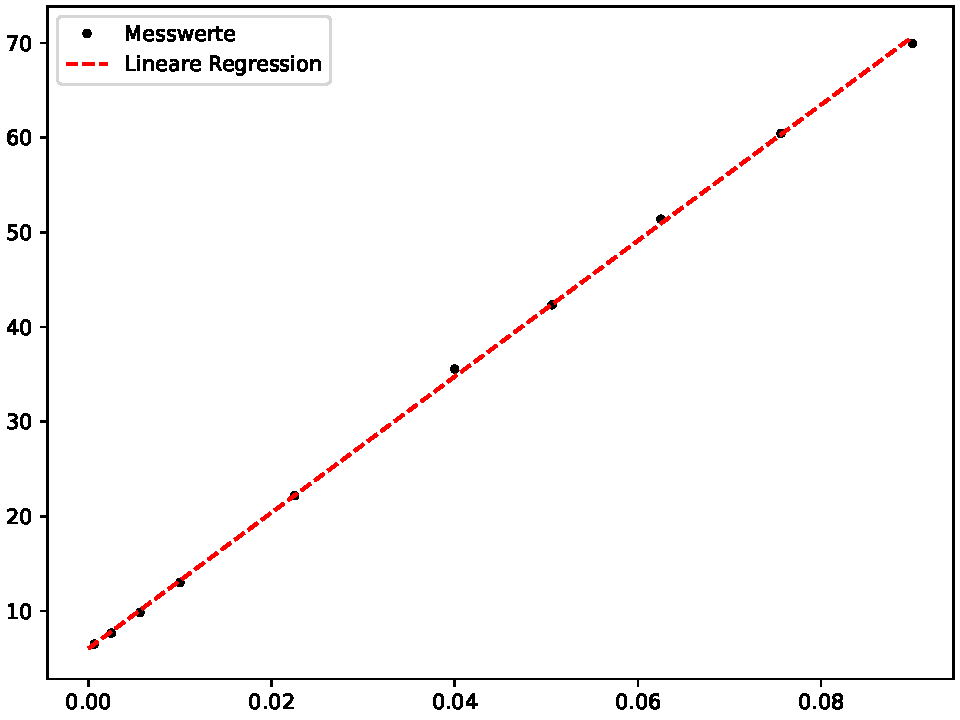
\includegraphics{plot.pdf}
  \caption{Abgebildet sind die Werte der Bildweite auf der y-Achse und die der Gegenstandsweite auf der x-Achse.}
  \label{fig:brenn}
\end{figure}

\subsection{Brennweitenbestimmung mit der Methode von Bessel}

Mithilfe von Gleichung \ref{eqn:brenn1} kann in diesem Fall die Brennweite über den Abstand der beiden Positionen der Linse $d$ und den Abstand zwischen Gegenstand und Schirm $e$ umformuliert werden als
\begin{equation}
  f=\frac{e^2-d^2}{4e} \text{.}
  \label{eqn:brenn2}
\end{equation}

\begin{table}
  \caption{Messwerte ohne einen Farbfilter.}
  \label{tab:bessel1}
  \centering
  \begin{tblr}{
    colspec={S[table-format=1.1] S[table-format=1.1] S[table-format=1.1] };
    row{1}={guard, mode=maths};
  }
  \toprule
  P_{L_1} \mathbin{/} \unit{\centi\meter}  & P_{L_2} \mathbin{/} \unit{\centi\meter} & P_S \mathbin{/} \unit{\centi\meter} \\
  \midrule
  38.5  &  54.6   &  70     \\
  37    &  60.7   &  75     \\
  36.6  &  66.4   &  80     \\
  36.1  &  71.6   &  85     \\
  35.9  &  76.7   &  90     \\
  35.8  &  82.1   &  95     \\
  35.8  &  87.2   &  100    \\
  35.4  &  92.5   &  105    \\
  35.2  &  97.5   &  110    \\
  35.2  &  102.7  &  115    \\  
  \bottomrule
  \end{tblr}
\end{table}

Daraus lassen sich $d$ und $e$ berechnen mit
\begin{align}
   & d=P_{L_2}-P_{L_1} \\
   & e=P_S-P_G \text{.}
\end{align}
Der errechnete Mittelwert für die Brennweite $f$ beträgt dann nach Gleichung \ref{eqn:brenn2} $\qty{9.80(0.06)}{\centi\meter}$

\begin{table}[H]
  \centering
  \label{tab:bessel2}
  \caption{Messwerte mit einem blauen Filter.}
  \begin{tblr}{
    colspec={S[table-format=1.1] S[table-format=1.1] S[table-format=1.1] };
    row{1}={guard, mode=maths};
    }
    \toprule
    P_{L_1} \mathbin{/} \unit{\centi\meter}  & P_{L_2} \mathbin{/} \unit{\centi\meter} & P_S \mathbin{/} \unit{\centi\meter} \\
    \midrule
    38.2  &  54.8  &  70  \\
    37.2  &  60.5  &  75  \\
    36.5  &  66.5  &  80  \\
    36.4  &  71.8  &  85  \\
    36.0  &  76.9  &  90  \\
    \bottomrule
  \end{tblr}
\end{table}


\begin{table}[H]
  \centering
  \label{tab:bessel3}
  \caption{Messwerte mit einem rotem Filter.}
  \begin{tblr}{
    colspec={S[table-format=1.1] S[table-format=1.1] S[table-format=1.1] };
    row{1}={guard, mode=maths};
    }
    \toprule
    P_{L_1} \mathbin{/} \unit{\centi\meter}  & P_{L_2} \mathbin{/} \unit{\centi\meter} & P_S \mathbin{/} \unit{\centi\meter} \\
    \midrule
    38.4  &  54.7  &  70 \\
    37.3  &  60.7  &  75 \\
    36.8  &  66.3  &  80 \\
    36.3  &  71.6  &  85 \\
    36.3  &  76.7  &  90 \\
    \bottomrule
  \end{tblr}
\end{table}

Nach der gleichen Methode, wie bei der Messung ohne Filter, wird die Brennweite der Linse bestimmt mit den Farbfiltern. Dabei ergeben sich Brennweiten von $f_b=\qty{9.75(0.06)}{\centi\meter}$ und $f_r=\qty{9.82(0.08)}{\centi\meter}$.


%Siehe \autoref{fig:plot} und \autoref{tab:tabelle}!


\subsection{Brennweitenbestimmung mit der Methode von Abbe}

